%!TEX root = ../report.tex

\begin{document}
    \chapter{AI Assisted Grading System}

	The best active learning strategies (query strategy, and seed selection), features extracted from the answers, and machine learning model which were determined from the experimental results were incorporated into a Graphical User Interface (GUI) to be used by teachers or professors while grading. Initially, the system queries the grades for certain percentage of the total answers from the human grader, and then displays the notebooks in 'question-wise' view. The purpose of question-wise view is to make the task of assessing the answers easier for the humans. This GUI along with the functionality of each of its components have been discussed below. 
	   
    \section{Software Architecture}
    
    	\begin{figure}[!htb]
    		\centering
    		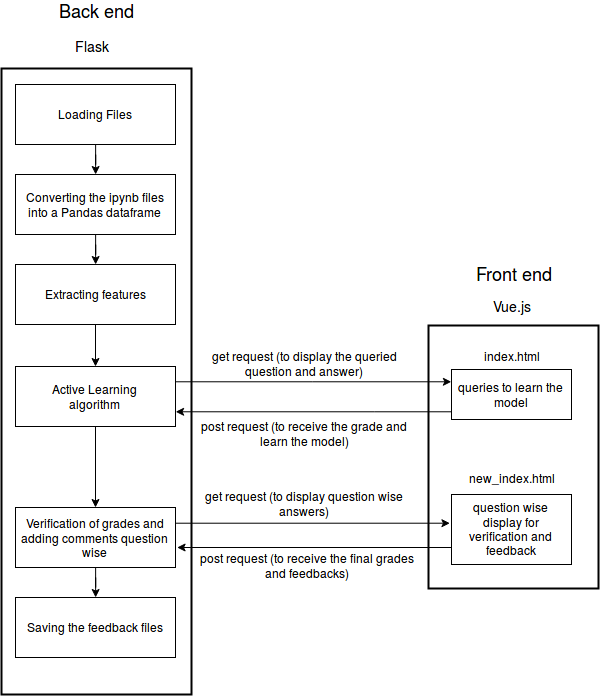
\includegraphics[scale=0.5]{images/gui_architecture}
    		\caption{Architecture of the AI-assisted grading system (GUI).}
    		\label{gui_architecture}
    	\end{figure}
	
	Fig \ref{gui_architecture} shows the architecture of the GUI implemented in this project. This system reads all the notebook files of the students from a specified directory, converts them into a Pandas dataframe, extracts the features from the answers needed for the machine learning algorithm, learns the model for the task of grading, gets the grades confirmed by a human and stores the grades along with human expert's feedbacks which is saved in another directory as Jupyter Notebook files. Tasks which include getting the notebook files, processing them through the machine learning algorithm and saving the grades with feedbacks occur in the backend while the display of the questions, answers, grades and feedbacks is taken care of by the front end. 
	
	The functionalities of the front end is done using \href{https://vuejs.org/}{Vue.js}. This framework is used to create a web-based graphical user interface using the JavaScript programming language. In addition, the elements of the page and the display features were written using HTML5 and CSS. \href{http://flask.pocoo.org/}{Flask} is a web development microframework which uses Python programming language. Since the machine learning models, and active learning settings were coded in Python, Flask came in handy to deal with the back end operations. 
	
	Once the notebooks are converted into the Pandas dataframe along with its features, the whole dataset is fed into the active learning algorithm. Fig \ref{gui_1} shows the stage where the queried answers appear in the GUI interface for the professor to grade. Certain percentage of the answers are queried from the professor in this manner and the model is learned using these grades. 
	
	\begin{figure}[!htb]
		\centering
		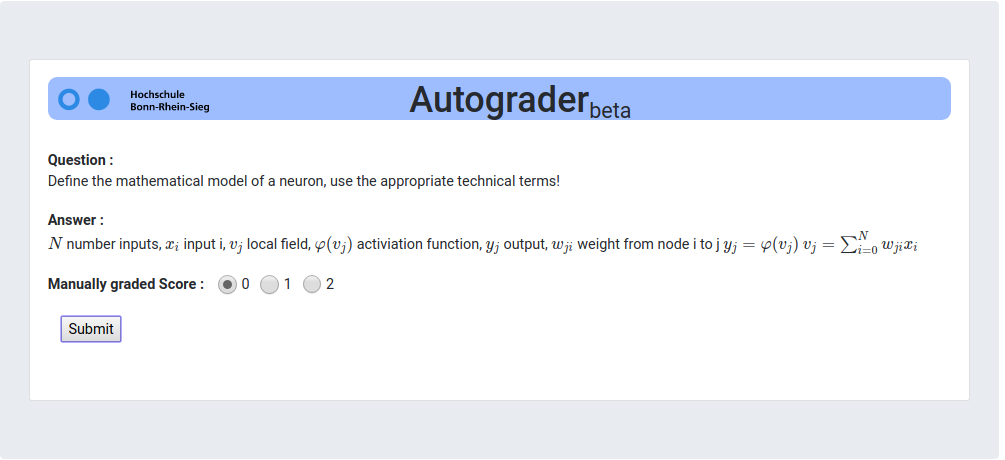
\includegraphics[scale=0.38]{images/gui_1}
		\caption{Querying stage of active learning in GUI.}
		\label{gui_1}
	\end{figure}  
	
	Once professor is done grading the initial set of answers queried through active learning, the autograded scores are displayed along with the answers question by question. Fig \ref{gui_2} shows this stage where all the students' answers to the first question for the professor to check. The autograded scores are binded to the manual grade radio buttons to ease the effort of professors while grading. The proffesors could simply leave the grades as it is if he thinks that they are right or he has the option to change the grades in the manual grade section. In addition, the professor can add further feedbacks by checking the relevant opinions given under every question. 
	
	\begin{figure}[!htb]
		\centering
		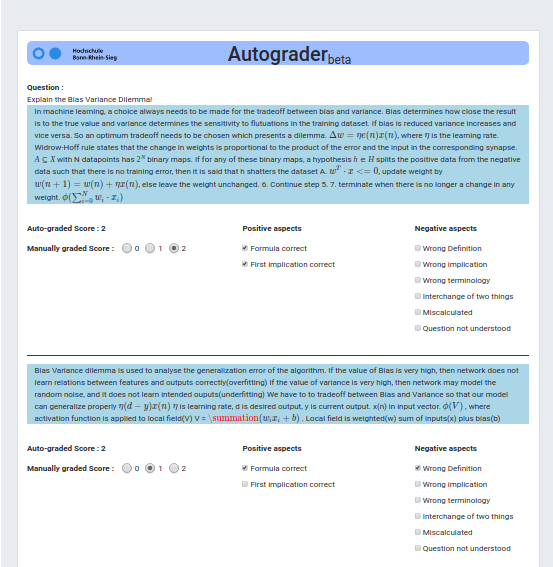
\includegraphics[scale=0.38]{images/gui_2}
		\caption{Question-wise view of answers after autograding stage.}
		\label{gui_2}
	\end{figure} 
	
	
	\begin{figure}[!htb]
		\begin{subfigure}[b]{0.5\textwidth}
			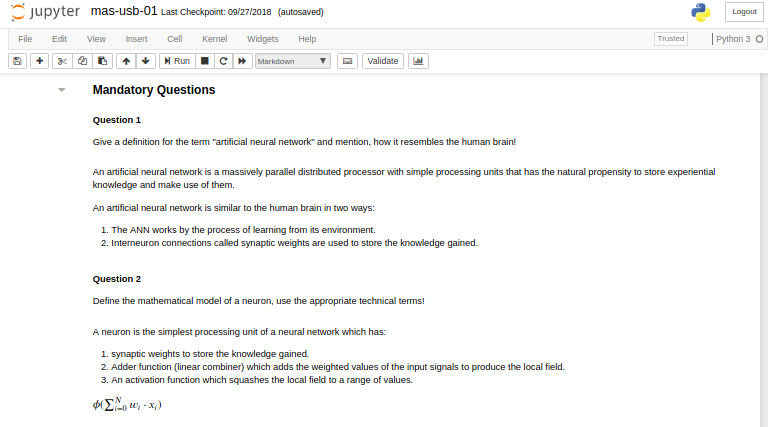
\includegraphics[width=\textwidth]{images/gui_4}
			\caption{Submitted student's answers in the notebook.}
			\label{gui_4}
		\end{subfigure}
		~
		\begin{subfigure}[b]{0.35\textwidth}
			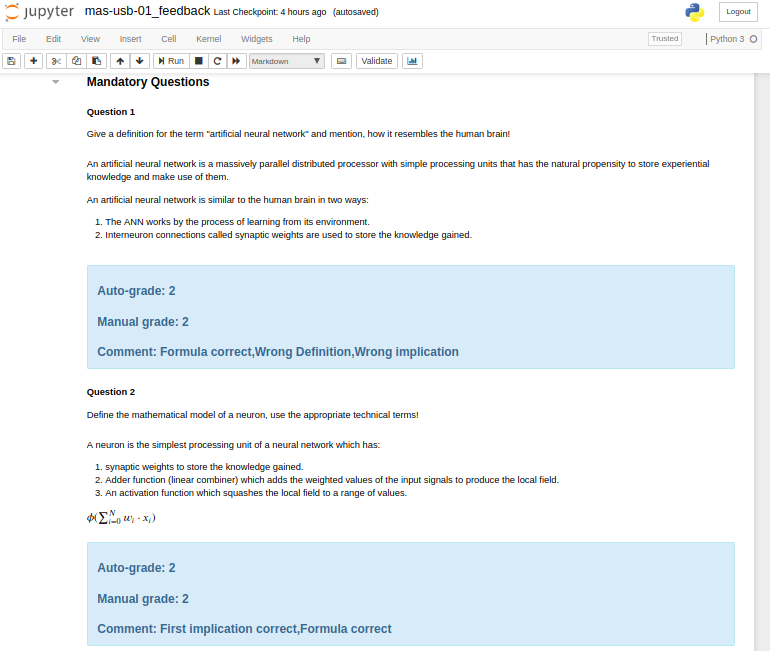
\includegraphics[width=\textwidth]{images/gui_3}
			\caption{Final format of the notebook with grades and feedbacks}
			\label{gui_3}
		\end{subfigure}
		~
		\caption{Initial and final versions of the notebook.}
	\end{figure}
	
	
	Once the professor has gone through all the questions, all the answers are saved back into jupyter notebook format. Fig \ref{gui_4} shows the initial format of the submitted students' answers in the notebook and Fig \ref{gui_3} shows the final format of the notebook once the final grades and feedbacks have been added to respective answers.
	
	\clearpage
	\section{User Experience}
	
	\subsection{Survey}
	
	Two users were asked to try grading a small percentage of answers and the survey answered by them is used to improve the interface and its functionalities. The survey questions and their answers by the users is given below.
	
	\vspace{3mm}
	
	\textbf{User 1}: 
	
	\begin{itemize}
		\item How easy is our grading to use ? \\
		In a scale of 1-10 , I would rate it as 6. 
		\item Did AI assisted grading reduce the effort of grading ? \\
		Yes. The difference was very clear. In manual grading I need to select the grades for all the answers and have to submit the grade. While in case of AI assisted grading most of the times I just need to verify the graded answer. Hence lots of effort for grading is reduced.
		\item How about the readability of Questions and answers ? \\
		The readability of question and answers was fine. Still, Various fonts can be tried to help the user find the better font for reading.
		\item How about the positioning and sizing of various elements (radio button,submit button)? \\
		Size of the radio button can be increased. Submit button can be on the right side as most of the users are right handed. 
		\item What features you think need to be added to enhance the experience ? \\
		Same question with different student answers can be displayed in a single page.
	\end{itemize}
	
	\textbf{User 2}:
	
	\begin{itemize}
		
		\item How easy is our grading to use ? \\
		In a scale of 1-10 , I would rate it as 7. 
		\item Did AI assisted grading reduce the effort of grading ? \\
		Yes. 
		\item How about the readability of Questions and answers ? \\
		Readability was satisfactory.
		\item How about the positioning and sizing of various elements (radio button,submit button)? \\
		Positioning can be improved a bit as I have to move the cursor here and there for selection. Instead it would be great if the movement of the cursor was in a sequential manner.
		\item What you think need to be added to enhance the experience ? \\
		Lot can be added to make the user feel comfortable. Various display options can be created. Autograding score can be embedded in other options other than radio button. Shortcuts can be created.
	\end{itemize}
	
	
	\subsection{Experiment: Number of clicks}
	
	A small experiment was conducted to realize the efficiency of using such an interface to grade the assignments with active learning in the background. One version of this experiment would be done by counting the total number of clicks while the grader grades all the answers for all the quesitons and the second version would be done with the support of active learning in the background, which computes the grades for all the questions once the learning phase is completed. The efficiency is judged by the reduction in the number of clicks required to grade all the answers in both the settings. 
	
	The experiments were done on all three datasets. All the students' answers in the notebooks are displayed question-wise in the active learning-free version. This would reflect the effort required to grade the assignments without using any assistance of any sort. In the version which uses active learning, the model is trained on the grades given by the grader for 25\% of the answers and then the answers are displayed question-wise along with the computed score for every answer. 
	
	The grader has the choice of changing the grade if he thinks that the suggested score by the model is wrong and this grade would be saved in a database for later converison into notebook. If the grader feels that the grade suggested by the model is reasonable, he could simply move on to the next student's answer to the same question. Viewing the answers question by question enables easier judgement of students' answers for the grader and faster grading. Random forest classifier with 100 trees and margin based uncertainty sampling was used in the learning process. The number of clicks made in both the learning-free version and learning assisted versions have been tabulated in Table \ref{clicks}.  
		
	\begin{table}[!htb]
		\centering
		\scalebox{0.75}{
			\begin{tabular}{|c|c|c|}
				\hline
				\textbf{Datasets}       & \textbf{Clicks with active learning} & \textbf{Clicks without active learning} \\ \hline
				\textbf{Neural network} & 338                                     & 680                                  \\ \hline
				\textbf{SemEval 2013}   & 3527                                    & 5104                                 \\ \hline
				\textbf{Mohler'11}      & 1386                                    & 2352                                 \\ \hline
			\end{tabular}}
			\caption{Number of clicks required to grade the answers with and without active learning.}
			\label{clicks}
		\end{table}
		
		As can be seen from the table above, the grading process assisted by active learning massively reduces the effort and time of the grader. In addition, the grader could spend more time in constructing useful feedbacks for the students by ticking the pertinent check boxes in the feedback section of the interface below every answer. 
	
	

\end{document}
